\section{Experimental validation}
\label{sec:exps}

We evaluated the performance of the above models on several real world weighted networks, both directed and undirected. Theirs characteristics and properties are summarized in Table \ref{table:corpus} and detailed descriptions are available in the online Koblenz network collection\footnote{http://konect.uni-koblenz.de/networks/}. For both astro-ph and hep-ph datasets, we used the cleaned versions available in the  graph-tool framework.
%The aim of these experiments is to illustrate the advantage of the online inference and to evaluate the performances of the models.
%This evaluation is based on a missing weight prediction task using the MSE score. 
 For all the datasets, we built a test set by extracting randomly 20 percent of the edges of the network and about the same amount of non-linked pairs of nodes\footnote{This selection, used in other studies, aims at simulating dense parts of the networks on which people usually focus.}. The remaining data constitutes the training set. We repeated this sampling 10 times with different seeds to cross validate our results. The average values (and standard deviations) computed on the ten sets are reported as final results.

In the remainder, for the MMSB, WMMSB and WMMSB-bg models, the gradient step parameters  $\tau$ and $\kappa$ were fixed respectively to  $1024$ and $0.5$, the burn-in period $T_{burnin}$ to $150$; for stratified sampling, $M$ was set to $50$, the size of $s_0^{i,m}, \, 1 \le m \le M$ being equal to the number of nodes to which $i$ is not connected to divided by $M$. For MMSB, the hyperparameters $\lambda_0$ and $\lambda_1$ were set to $0.1$. For WMMSB, $r$ and $p$ were set to $1$ and $1/2$ respectively, whereas for WMMSB-bg the hyperparameters were set to  $c_0=10$, $r_0=1$, $c=100$ and $\epsilon=10^{-6}$. For all three models, the latent-class hyperparameters $\alpha_k, \, 1 \le k \le K$ are set to $\frac{1}{K}$. The implementation of these models is available online\footnote{https://github.com/***/*** (anonymized)}. For deciding when to stop the inference process, 10\% of the training set used serves as a validation set on which the log-likelihood is computed after each minibatch iteration. When the increase of the log-likelihood, averaged over the last 20 measures, is less than 0.001, the inference is stopped. The log-likelihood of a given set of observations $\D_{set}$  is given by:
%
\begin{equation*}
\log p(\D_{set}) = \sum_{i,j \in \D_{set}} \log p(y_{ij} | \phih_{kk'}) p(k|\thetah_i) p(k'|\thetah_j).
%\log p(\D_{test}) = \sum_{i,j \in \D_{test}} \log p(y_{ij} | \phih_{kk'}) p(k|\thetah_i) p(k'|\thetah_j)
\end{equation*}
%

Predicting links and predicting weights on links are two different tasks, and there is no guarantee that a model performing well on one task will perform well on the other. Even though we focus in this study on the weight prediction problem, we still want, for completeness reasons, to illustrate the behavior of the different models on the link prediction task.

\subsection{Link prediction}

\begin{table*}[t]
\centering
	
\caption{AUC-ROC performance comparaison of the models. Each model has 2 columns corresponding to two subsamples of the full training set. The subsamble contains either 10 or 100 percent of the edges in the trainin set, and there are inclusive. The AUC value is performed on the testing set build from the initial dataset by extracting 20 percent of the edges and about the the same amount of non-edge. 
For each dataset we randomly build a unique training and testing set shared by all the model. The scores are averaged on 10 independents trials (for each trials we build a unique traning and testing set.) and scaled by a factor $10^{3}$ in the table. We bold the best results w.r.t the training set of 10 percent and we underline the best results w.r.t to the training set of 80 percent. The results show that the MMSB and WMMSB-bg with our inferenc scheme outperform SBM and WSBM when the number of observation is low. Furthermore WMMSB-bg outperforms MMSB on most of the datasets.}

%\resizebox{12cm}{!}{
\resizebox{\textwidth}{!}{

\begin{tabular}{lllll|llll}
\toprule
&   \multicolumn{2}{c}{MMSB} &   \multicolumn{2}{c}{WMMSB-bg} &   \multicolumn{2}{c}{SBM} & \multicolumn{2}{c}{WSBM}   \\
\cmidrule(l){2-3} \cmidrule(l){4-5} \cmidrule(l){6-7}\cmidrule(l){8-9}  & 10 & 100 & 10 & 100 & 10 &  100 & 10 & 100   \\
%\hline
\midrule                              
astro-ph        &  \textbf{708} $\pm$ 3    & \underline{716} $\pm$ 11          & 700 $\pm$ 30            &  710 $\pm$ 18   &   594 $\pm$ 16   &  701 $\pm$ 6               &   588 $\pm$ 12           & 705 $\pm$ 5  \\
hep-th          &  \textbf{617} $\pm$ 11   & 675 $\pm$ 8           & 579 $\pm$ 12            &  676 $\pm$ 8    &   480 $\pm$ 9    &  \underline{779} $\pm$ 1               &   497 $\pm$ 29            & 716 $\pm$ 9  \\
moreno\_names   &  680 $\pm$ 72            & 738 $\pm$ 33          & \textbf{707} $\pm$ 29   &  739 $\pm$ 7    &   571 $\pm$ 29   &  \underline{862} $\pm$ 7               &   588 $\pm$ 25            & 862 $\pm$ 10 \\
fb\_uc          &  732 $\pm$ 127           & 784 $\pm$ 14          & \textbf{827} $\pm$ 8    &  850 $\pm$ 20   &   726 $\pm$ 20   &  \underline{902} $\pm$ 2               &   787 $\pm$ 15            & 896 $\pm$ 2  \\
digg\_reply     &  485 $\pm$ 178           & 482 $\pm$ 204         & \textbf{651} $\pm$ 127  &  744 $\pm$ 15   &   551 $\pm$ 47   &  728 $\pm$ 26              &   584 $\pm$ 34            & 714 $\pm$ 17 \\
slashdot        &  519 $\pm$ 193           & 634 $\pm$ 181         & \textbf{820} $\pm$ 6    &  791 $\pm$ 11   &   721 $\pm$ 66   &  830 $\pm$ 16              &   699 $\pm$ 79            & \underline{833} $\pm$ 13 \\
enron           &  459 $\pm$ 289           & 529 $\pm$ 256         & \textbf{875} $\pm$ 14   &  835 $\pm$ 8    &   870 $\pm$ 80   &  799 $\pm$ 20              &   866 $\pm$ 45            & \underline{842} $\pm$ 51 \\
wiki-link       &  491 $\pm$ 242           & 432 $\pm$ 185         & 739 $\pm$ 73            &  785 $\pm$ 8    &   848 $\pm$ 4    &  \underline{925} $\pm$ 2               &   \textbf{853} $\pm$ 4    & 914 $\pm$ 4  \\
prosper-loans   &  548 $\pm$ 284           & 434 $\pm$ 274         & \textbf{752} $\pm$ 11   &  \underline{727} $\pm$ 30   &   466 $\pm$ 57   &  500 $\pm$ 4               &   455 $\pm$ 44  	       & 505 $\pm$ 5  \\

\bottomrule
\end{tabular}


}


          
          
          





% 5 20 100

%&   \multicolumn{3}{c}{MMSB} &   \multicolumn{3}{c}{WMMSB-bg} &   \multicolumn{3}{c}{SBM} & \multicolumn{3}{c}{WSBM}     \\
%\cmidrule(l){2-4} \cmidrule(l){5-7} \cmidrule(l){8-10}\cmidrule(l){11-13}  & 5 & 20 & 100 & 5 & 20 & 100 & 5 & 20 & 100 & 5 & 20 & 100   \\

%astro-ph        &  686 $\pm$ 7    & 720 $\pm$ 8    & 716 $\pm$ 11   & 684 $\pm$ 25 & 690 $\pm$ 40  &  710 $\pm$ 18   &    505 $\pm$ 9  &  627 $\pm$ 5   &  701 $\pm$ 6   &  538 $\pm$ 31  &    626 $\pm$ 9   & 705 $\pm$ 5  \\
%hep-th          &  583 $\pm$ 13   & 655 $\pm$ 6    & 675 $\pm$ 8    & 558 $\pm$ 9  & 630 $\pm$ 21  &  676 $\pm$ 8    &   498 $\pm$ 6   &  506 $\pm$ 13  &  779 $\pm$ 1   &  513 $\pm$ 24   &    545 $\pm$ 29  & 716 $\pm$ 9  \\
%moreno\_names   &  674 $\pm$ 43   & 740 $\pm$ 18   & 738 $\pm$ 33   & 664 $\pm$ 39 & 697 $\pm$ 33  &  739 $\pm$ 7    &   478 $\pm$ 59  &  698 $\pm$ 25  &  862 $\pm$ 7   &  457 $\pm$ 38   &    709 $\pm$ 9   & 862 $\pm$ 10 \\
%fb\_uc          &  723 $\pm$ 109  & 728 $\pm$ 140  & 784 $\pm$ 14   & 790 $\pm$ 20 & 846 $\pm$ 11  &  850 $\pm$ 20   &   590 $\pm$ 43  &  846 $\pm$ 13  &  902 $\pm$ 2   &  679 $\pm$ 27   &    855 $\pm$ 7   & 896 $\pm$ 2  \\
%digg\_reply     &  491 $\pm$ 150  & 486 $\pm$ 195  & 482 $\pm$ 204  & 667 $\pm$ 73 & 723 $\pm$ 31  &  744 $\pm$ 15   &   528 $\pm$ 51  &  677 $\pm$ 13  &  728 $\pm$ 26  &  554 $\pm$ 22   &    659 $\pm$ 26  & 714 $\pm$ 17 \\
%slashdot        &  537 $\pm$ 177  & 538 $\pm$ 186  & 634 $\pm$ 181  & 801 $\pm$ 13 & 822 $\pm$ 6   &  791 $\pm$ 11   &   712 $\pm$ 66  &  775 $\pm$ 72  &  830 $\pm$ 16  &  731 $\pm$ 64   &    733 $\pm$ 28  & 833 $\pm$ 13 \\
%enron           &  555 $\pm$ 300  & 576 $\pm$ 301  & 529 $\pm$ 256  & 862 $\pm$ 15 & 876 $\pm$ 9   &  835 $\pm$ 8    &   900 $\pm$ 3   &  898 $\pm$ 39  &  799 $\pm$ 20  &  887 $\pm$ 48   &    916 $\pm$ 29  & 842 $\pm$ 51 \\
%wiki-link       &  389 $\pm$ 192  & 505 $\pm$ 230  & 432 $\pm$ 185  & 749 $\pm$ 43 & 725 $\pm$ 87  &  785 $\pm$ 8    &   517 $\pm$ 59  &  870 $\pm$ 4   &  925 $\pm$ 2   &  592 $\pm$ 159  &    871 $\pm$ 2   & 914 $\pm$ 4  \\
%prosper-loans   &  569 $\pm$ 300  & 622 $\pm$ 233  & 434 $\pm$ 274  & 736 $\pm$ 54 & 746 $\pm$ 28  &  727 $\pm$ 30   &   439 $\pm$ 97  &  503 $\pm$ 74  &  500 $\pm$ 4   &  472 $\pm$ 59   &    504 $\pm$ 39  & 505 $\pm$ 5  \\

                     
                     
                     
                     
                     
                     
                     
                     
                     
               
               
                                                                                                                                        
                     
                                                                                                                                           
                     
                     
                                                                                                                                           
                     
                     
                     
                                                                                                                     









\label{table:roc}
\end{table*}

In addition to the proposed mixed-membership models, we consider here two standard link prediction models, the stochastic block model, referred to as SBM, and its weighted extension, referred to as WSBM. We use the most recent version of these two models, namely the microcanonical stochastic block model implementation of \cite{peixoto2018nonparametric}, which relies on an efficient MCMC inference method. In all models, the number of classes is set to $K=10$ (as illustrated below, the choice of the number of latent classes, in between 10 and 50, does not have an important impact on these models).

As usual, the missing link prediction task is evaluated with the AUC-ROC score. For weighted models, we simply predict here a link through the probability that an edge exists between two unobserved nodes $(i,j)$ belonging to the test set, namely:
\[
p(y_{ij} \geq 1 | \Bs{\Thetah}, \Bs{\Phih}) = 1 - \sum_{1 \le k,k' \le K} \thetah_{ik} \thetah_{jk'} e^{-\phih_{kk'}}
\]

%Variational inference, used here for MMSB models, and MCMC, used for SBM models, lead to different performance, the latter usually yielding better models than the former \cite{asuncion2009smoothing}. Indeed, despite the fact that the MMSB models considered here rely on more realistic assumptions regarding the distribution of nodes over latent classes, the approximations made on the likelihood for scalable inference purposes penalize MMSB models when it comes to prediction accuracy. This said, the strong averaging step of the stochastic gradient descent allows for faster convergence so that, as the models are more realistic, they may yield better performance when the amount of training data is limited. This is indeed what we observe in practice.

Table~\ref{table:roc} summarizes the results obtained with the above mentioned models when using 10\% and 100\% of the training data. As one can note, when the complete training set is used (100 \%), SBM outperforms WSBM on 5 datasets and is overall the best performing model. This can be attributed to the fact that SBM directly aims at predicting links, unlike the weighted models, and does so via MCMC inference, which is known to yield accurate estimate when there is sufficient data. The mixed-membership family does not yield good results in this setting (100\%) and is only interesting, in particular via WMMSB-bg, on four datasets (astro\_ph, digg\_reply, enron, and prosper\_loans). Within this family, WMMSB-bg outperforms the other models on seven datasets (hep-th, moreno\_names, fb\_uc, digg\_reply, slashdot, wiki-link and prosper\_loans). For this reason, we will not use its simpler version, WMMSB, in the remainder of this study. Lastly, there is however an important degradation for SBM models when only 10\% of the training set is used. Mixed-membership stochastic block models are more stable in this case (except on enron and wiki-link), indicating that the stochastic variational inference used in these models is appropriate with relatively few data. %Lastly, among the models proposed in this study, WMMSB-bg outperforms WMMSB. We rely, for this reason, on the former in the remainder of the study.

\subsection{Weight prediction}

For this task, in addition to the previous models, we consider three other stochastic block models from \cite{aicher2014learning}, among which two are weighted. These models are based on a generic variational inference scheme with several kernels: a Bernoulli kernel for the model referred to as SBM-ai, a Normal kernel for the model referred to as WSBM-ai-n, and a Poisson kernel for the model referred to as WSBM-ai-p. Lastly, we also consider the Edge Partition Model (EPM) proposed in~\cite{zhou2015} (see Section~\ref{sec:rl}), the inference of which relies on MCMC.

For both WMMSB-bg and EPM, we used the inferred posterior distribution to estimate the missing weights by:
%
\begin{equation}\label{eq:assign}
\hat y_{ij} | \Bs{\Thetah}, \Bs{\Phih} = \sum_{1 \le k,k' \le K} \thetah_{ik} \thetah_{jk'} \phih_{kk'}
\end{equation}
%
%Note that the Zero Truncated Poisson version of WMMSB-bg would lead to:
%%
%\[
%\hat y_{ij} | \Bs{\Thetah}, \Bs{\Phih} = \sum_{kk'} \thetah_{ik} \thetah_{jk'} \frac{\phih_{kk'}}{(1 - \exp(-\phih_{kk'}))}
%\]
%%
%In practice however, even though the latter version is more appropriate, we have not seen any significant difference between the two versions and present only the results obtained with the former so as to be on the same setting as the other models.
%
Since the stochastic block models have been primarily designed for solving the link prediction task, we do not have a posterior distribution adapted for weight prediction. Therefore, we used an estimation of the average weight value in each interaction based on the observed data. More precisely, let $N_k$ denote the number of nodes assigned to class $k$ by the model in the training set. The prediction of the weight on the link between two nodes $i$ and $j$ of the test set, respectively of class $k$ and $k'$, is given by:
%
\[
\hat y_{ij} | i \in k, j \in k' = \sum_{(i',j') \in \mathcal{T}_s, i' \in k, j' \in k} \frac{y_{i'j'}}{N_k N_{k'}},
\]
%
where $i \in k$ means that node $i$ was assigned to class $k$ by the model and $\mathcal{T}_s$ denotes the training set.
 
The same method is used for the weighted stochastic block models WSBM, WSBM-ai, WSBM-ai-n and WSBM-ai-p as this method yielded even better results than the one directly making use of the expectation of $y_{ij}$ as in Eq.~\ref{eq:assign}.

\begin{table*}[t]
\centering
	\caption{Comparison of models in terms of MSE on different networks for $K=10$.}

\resizebox{\textwidth}{!}{
\begin{tabular}{lllllllll}
\hline
               & MMSB-scvb          & WMMSB-bg                    & EPM                        & SBM-ai             & WSBM-ai-n          & WSBM-ai-p          & SBM-gt             & WSBM-gt              \\                              
\hline                                                                                                                                                                             
 astro-ph      & 36.94 $\pm$ 1.38   & \textbf{25.04} $\pm$ 2.73   & 36.93 $\pm$ 1.43           & 36.85 $\pm$ 1.24   & 36.65 $\pm$ 1.39   & 36.29 $\pm$ 1.82   & 38.22 $\pm$ 1.62   & 36.94 $\pm$ 1.83     \\
 enron         & 119.53 $\pm$ 9.8   & \textbf{103.85} $\pm$ 7.09  & 122.73 $\pm$ 8.86          & 127.13 $\pm$ 7.87  & 130.65 $\pm$ 13.83 & 133.51 $\pm$ 12.11 & 115.25 $\pm$ 8.37  & 126.18 $\pm$ 11.12   \\
 fb\_uc        & 32.92 $\pm$ 2.48   & \textbf{23.85} $\pm$ 2.37   & 25.82  $\pm$ 2.17          & 31.80 $\pm$ 2.95   & 35.95 $\pm$ 3.02   & 34.50 $\pm$ 2.84   & 30.85 $\pm$ 4.31   & 30.76 $\pm$ 4.44     \\
 hep-th        & 235.92 $\pm$ 18.53 & \textbf{148.03} $\pm$ 14.22 & 242.28 $\pm$ 16.9          & 246.93 $\pm$ 27.22 & 242.53 $\pm$ 13.98 & 235.99 $\pm$ 24.01 & 237.81 $\pm$ 21.56 & 224.07 $\pm$ 30.74   \\
 wiki-link     & 12.08 $\pm$ 0.49   & \textbf{9.48} $\pm$ 0.32    & 11.26  $\pm$ 0.15          & 11.86 $\pm$ 0.17   & 11.82 $\pm$ 0.48   & 12.01 $\pm$ 0.25   & 11.99 $\pm$ 0.19   & 11.68 $\pm$ 0.56     \\
 moreno\_names & 12.30 $\pm$ 2.01   & 7.93 $\pm$ 1.58             & \textbf{6.16} $\pm$ 0.99   & 12.92 $\pm$ 3.29   & 13.32 $\pm$ 2.97   & 10.59 $\pm$ 1.97   & 10.00 $\pm$ 2.62   & 9.53 $\pm$ 2.71      \\
 digg-reply    & 4.06 $\pm$ 0.01    & \textbf{0.48} $\pm$ 0.07    & 4.03   $\pm$ 0.02          & 4.06 $\pm$ 0.02    & 4.05 $\pm$ 0.01    & 4.05 $\pm$ 0.01    & 4.04 $\pm$ 0.03    & 4.05 $\pm$ 0.02      \\
 prosper-loans & 4.09 $\pm$ 0.01    & \textbf{0.33} $\pm$ 0.36    & 3.88   $\pm$ 0.01          & 4.08 $\pm$ 0.0     & 4.09 $\pm$ 0.0     & 4.08 $\pm$ 0.0     & 3.95 $\pm$ 0.01    & 3.95 $\pm$ 0.01      \\
 slashdot      & 4.33 $\pm$ 0.01    & \textbf{0.73} $\pm$ 0.08    & 4.24   $\pm$ 0.01          & 4.32 $\pm$ 0.01    & 4.33 $\pm$ 0.01    & 4.35 $\pm$ 0.02    & 4.27 $\pm$ 0.01    & 4.28 $\pm$ 0.01      \\
\hline
\end{tabular}
}


\label{table:mse}
\end{table*}

\begin{figure*}[ht]
\centering
	\begin{subfigure}
     \centering
         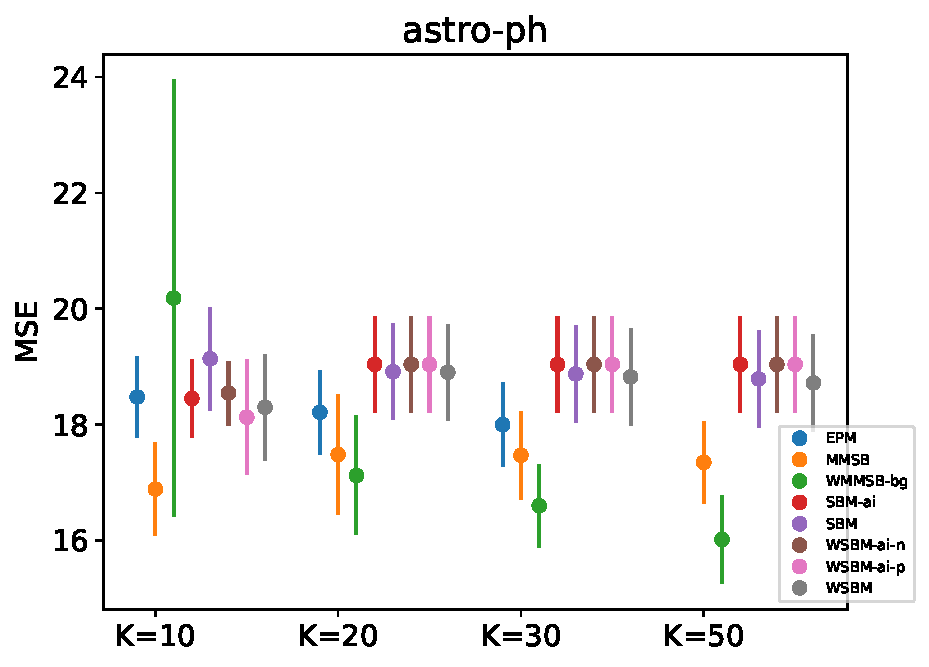
\includegraphics[width=0.32\textwidth]{fig2/astro-ph_wsim3_evo2__}
\end{subfigure}
\begin{subfigure}
         \centering
      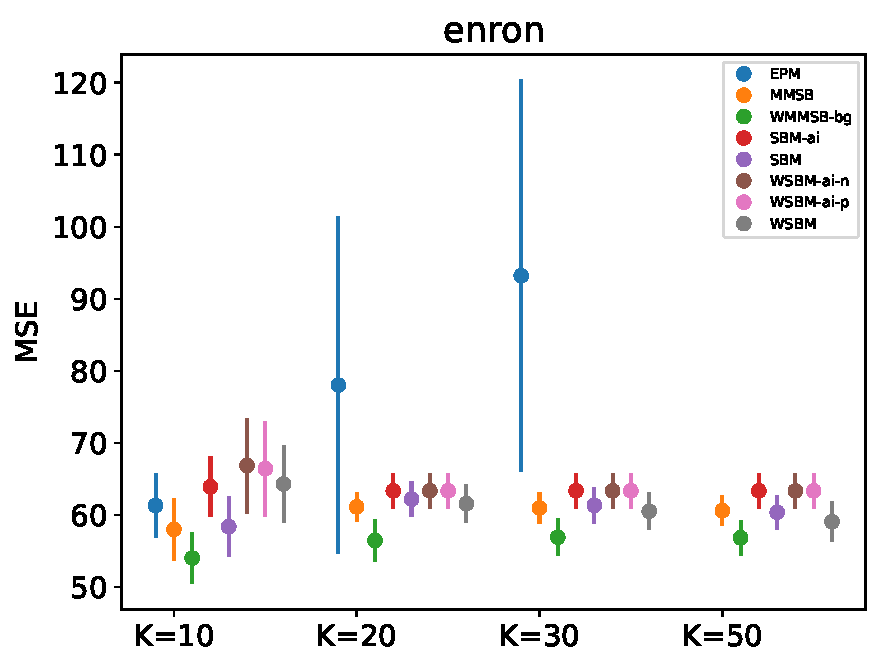
\includegraphics[width=0.32\textwidth]{fig2/enron_wsim3_evo2__}   
\end{subfigure}  
\begin{subfigure}
         \centering          
      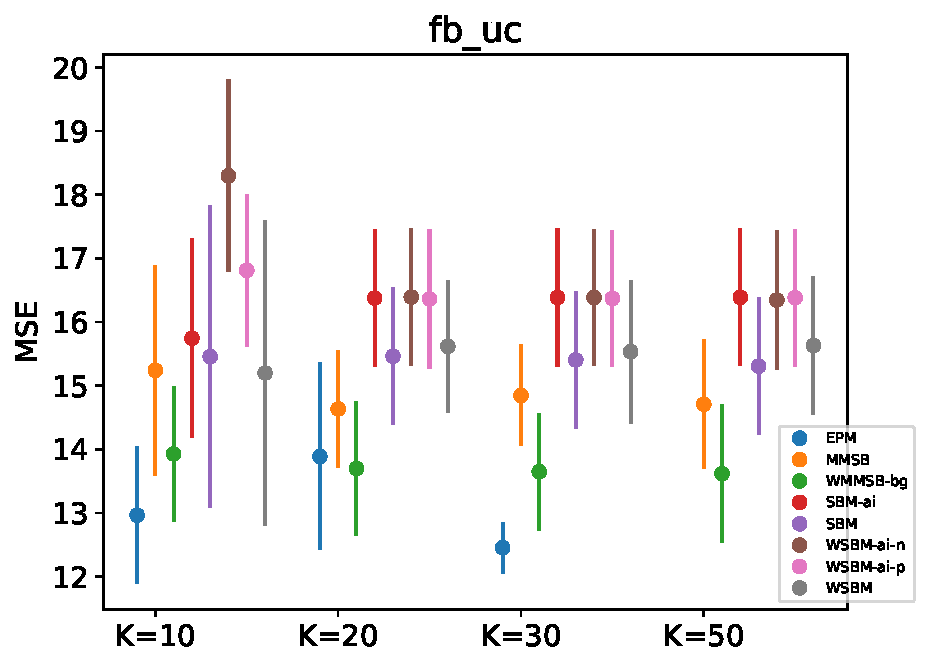
\includegraphics[width=0.32\textwidth]{fig2/fb_uc_wsim3_evo2__}
\end{subfigure}  
\caption{Impact of the number of classes on the performance of the different models, from $K=10$ to $K=50$, on astro\_ph, enron and fb\_uc.}


   \label{fig:k_evolv}
\end{figure*}

Table \ref{table:mse} provides the mean squared error (MSE) scores for the different models and for all networks. For all models, the number of latent classes $K$ is set to 10.
%To evaluate the ability of the models to reconstruct the missing weights, we compute the MSE only on the missing edges of the test data. Although the models are also able to predict the presence or absence of edges,  we considered that the question of recovering the edges structure should be addressed separately by a link prediction method. 
As one can note, the overall best performing model is WMMSB-bg, which yields the best results on 8 out of 9 datasets. MMSB, the other representative of the mixed-membership family, yields the best result on astro\_ph while EPM is the best performing model on fb\_uc and moreno\_names, even though the difference with respect to WMMSB-bg on fb\_uc is not large. Overall, the stochastic block models and their weighted versions do not perform well compared to WMMSB-bg (and to a lesser extent to EPM), which shows the importance of the soft class assignment mechanism present in mixed-membership models. 

%outperforms all the other models on the different datasets except for the network moreno\_names. 
%The fact that this network is the only one in the category of linguistic network and that it is relatively small could explain this result. \textbf{CL : je ne suis pas d'accord avec phrase suivante} EPM outperforms other models, apart from WMMSB-bg. The other models expose comparable results.

\subsubsection{Impact of the number of classes} 

Figure \ref{fig:k_evolv} displays, for three datasets, the evolution of the MSE scores when the number of latent classes, $K$, varies from 10 to 50  (additional results are provided in Appendix~\ref{app:K}). As one can see, the results are relatively stable for all models. This is particularly true for the WMMSB-bg model. Note that the EPM model, due to its reliance on MCMC for inference, was not able to handle as many as 50 latent classes in a reasonable time (see below). This model also displays high variance when $K$ increases on the enron network, reflecting the fact that the variance of the weights in this network is by far the most important (see Table~\ref{table:corpus}).

%%%%%%%%%%%%%%%%%%%%%%%%%%%%%%%%%%%%%%%%%%%%%%%%%%%%%%%%
%%%% Timing performance
%%%%%%%%%%%%%%%%%%%%%%%%%%%%%%%%%%%%%%%%%%%%%%%%%%%%%%%%
\begin{table*}[t]
\centering
	\caption{Comparison of models in terms of inference time, in hour, on different datasets for $K=10$. Results are averaged over 10 runs $\pm$ standard deviation. }

\vspace{0.2cm}

\resizebox{\textwidth}{!}{
\begin{tabular}{lllllllll}
\hline
              & MMSB          & WMMSB-bg           & EPM                          & SBM-ai               & WSBM-ai-n        & WSBM-ai-p          & SBM                  & WSBM                  \\
\hline                                                                                                                                                                  
astro-ph      & 0.09 $\pm$ 0.02    & 0.07 $\pm$ 0.02    & \textit{1.08}  $\pm$ 0.01    & 0.08 $\pm$ 0.01      & 0.07 $\pm$ 0.01  & 0.08 $\pm$ 0.02    & \textbf{0.01} $\pm$ 0.01     & 0.03 $\pm$ 0.01          \\
hep-th        & 0.05 $\pm$ 0.01    & 0.08 $\pm$ 0.04    & \textit{0.26}  $\pm$ 0.01    & 0.02 $\pm$ 0.01      & 0.02 $\pm$ 0.01  & 0.02 $\pm$ 0.01    & \textbf{0.01} $\pm$ 0.01     & 0.01 $\pm$ 0.01          \\
moreno\_names & 0.02 $\pm$ 0.02    & 0.01 $\pm$ 0.01    & \textit{0.02}  $\pm$ 0.01    & 0.01 $\pm$ 0.01      & 0.01 $\pm$ 0.01  & 0.01 $\pm$ 0.01    & \textbf{0.01} $\pm$ 0.01     & 0.01 $\pm$ 0.01         \\
fb\_uc        & 0.01 $\pm$ 0.01    & 0.02 $\pm$ 0.01    & \textit{0.02}  $\pm$ 0.01    & 0.01 $\pm$ 0.01      & 0.01 $\pm$ 0.01  & 0.01 $\pm$ 0.01    & \textbf{0.01} $\pm$ 0.01     & 0.01 $\pm$ 0.01           \\
digg-reply    & 0.51 $\pm$ 0.30    & 0.71 $\pm$ 0.27    & \textit{4.69}  $\pm$ 0.04    & 0.15 $\pm$ 0.01      & 0.14 $\pm$ 0.01  & 0.15 $\pm$ 0.01    & \textbf{0.02} $\pm$ 0.01     & 0.06 $\pm$ 0.01          \\
slashdot      & 1.27 $\pm$ 0.24    & 1.51 $\pm$ 0.48    & \textit{12.98} $\pm$ 1.26    & 0.39 $\pm$ 0.03      & 0.36 $\pm$ 0.03  & 0.39 $\pm$ 0.04    & \textbf{0.04} $\pm$ 0.01     & 0.08 $\pm$ 0.01          \\
enron         & 1.52 $\pm$ 0.62    & 1.29 $\pm$ 0.61    & \textit{25.03} $\pm$ 0.03    & 1.13 $\pm$ 0.08      & 1.04 $\pm$ 0.05  & 1.00 $\pm$ 0.16    & \textbf{0.10} $\pm$ 0.01     & 0.22 $\pm$ 0.01          \\
wiki-link     & 2.15 $\pm$ 0.50    & 1.67 $\pm$ 0.34    & \textit{25.10} $\pm$ 0.03    & 1.38 $\pm$ 0.16      & 1.48 $\pm$ 0.08  & 1.58 $\pm$ 0.33    & \textbf{0.29} $\pm$ 0.01     & 0.63 $\pm$ 0.05          \\
prosper-loans & 0.87 $\pm$ 0.24    & 1.71 $\pm$ 0.78    & \textit{25.13} $\pm$ 0.03    & 1.64 $\pm$ 0.09      & 1.62 $\pm$ 0.10  & 1.64 $\pm$ 0.20    & \textbf{1.38} $\pm$ 0.09     & 3.04 $\pm$ 0.22          \\
\hline
\end{tabular}
}

\label{table:time}
\end{table*}

\subsubsection{Inference time} 

\begin{figure*}[t]
\centering
	%

\begin{subfigure}
     \centering
         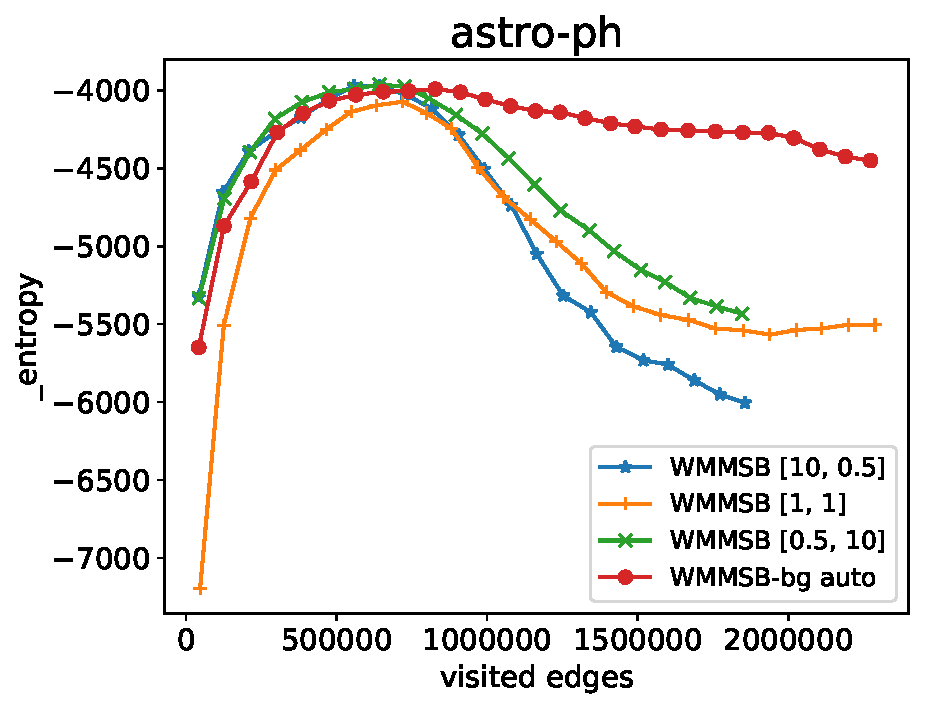
\includegraphics[width=0.32\textwidth]{fig/astro-ph_fig__entropy}
\end{subfigure}
\begin{subfigure}
         \centering
      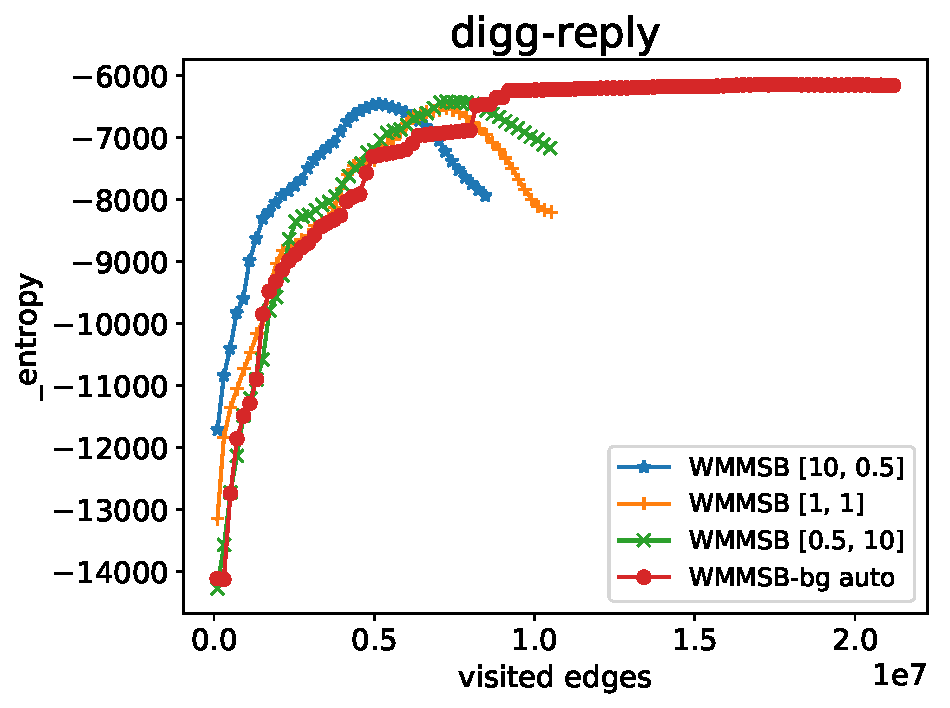
\includegraphics[width=0.32\textwidth]{fig/digg-reply_fig__entropy}               
\end{subfigure}                                                                          
\begin{subfigure}                                                                        
         \centering                                                                      
      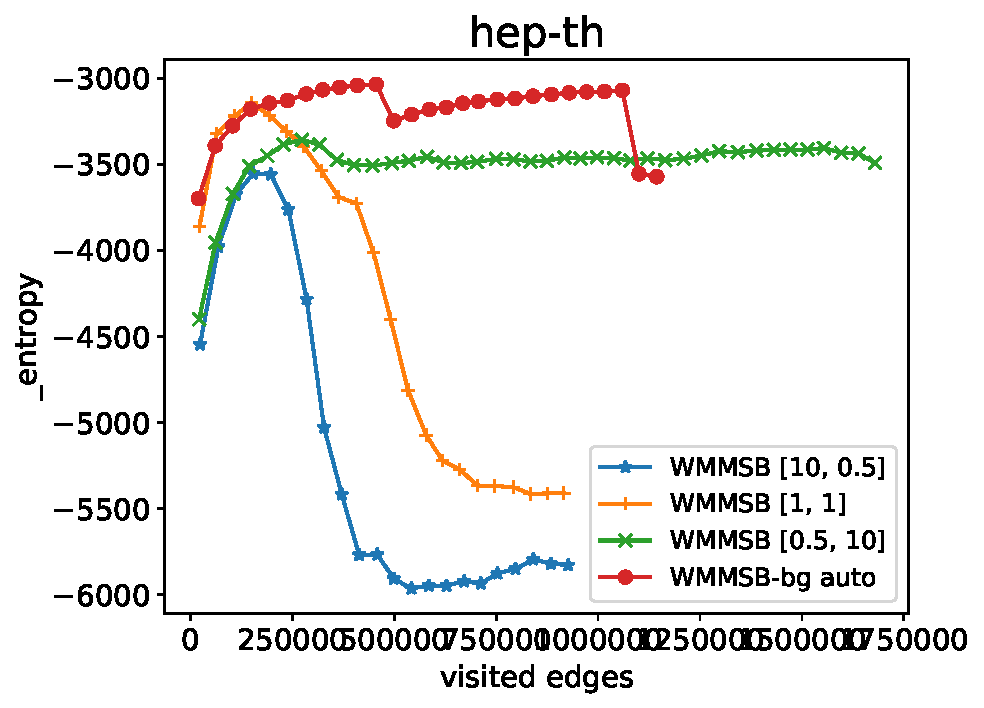
\includegraphics[width=0.32\textwidth]{fig/hep-th_fig__entropy}
\end{subfigure}                                                                          
\begin{subfigure}                                                                        
     \centering                                                                          
         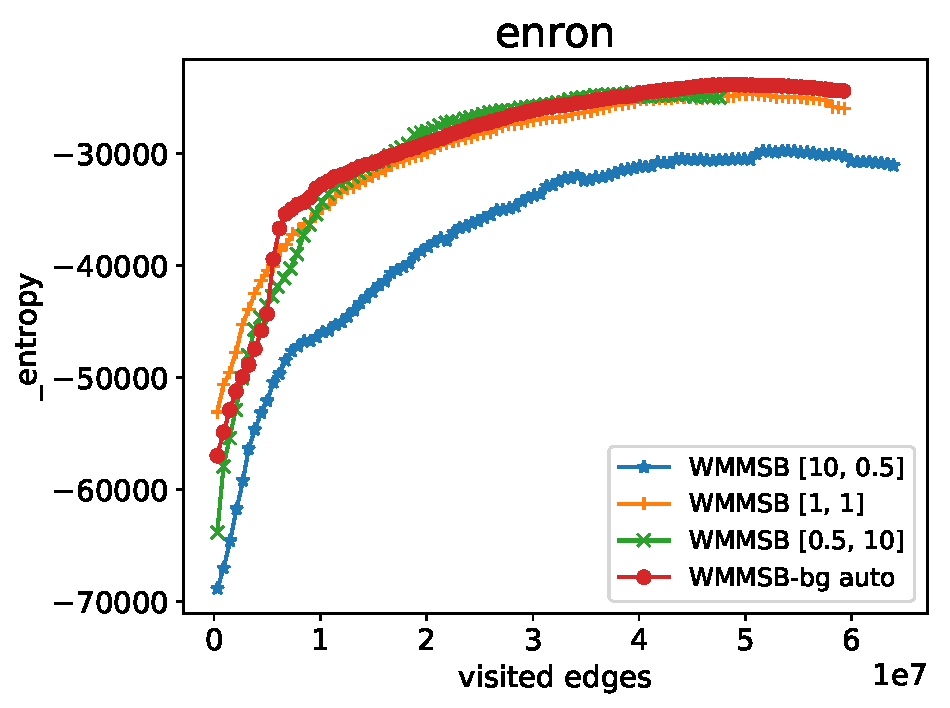
\includegraphics[width=0.32\textwidth]{fig/enron_fig__entropy}
\end{subfigure}
\begin{subfigure}
         \centering
      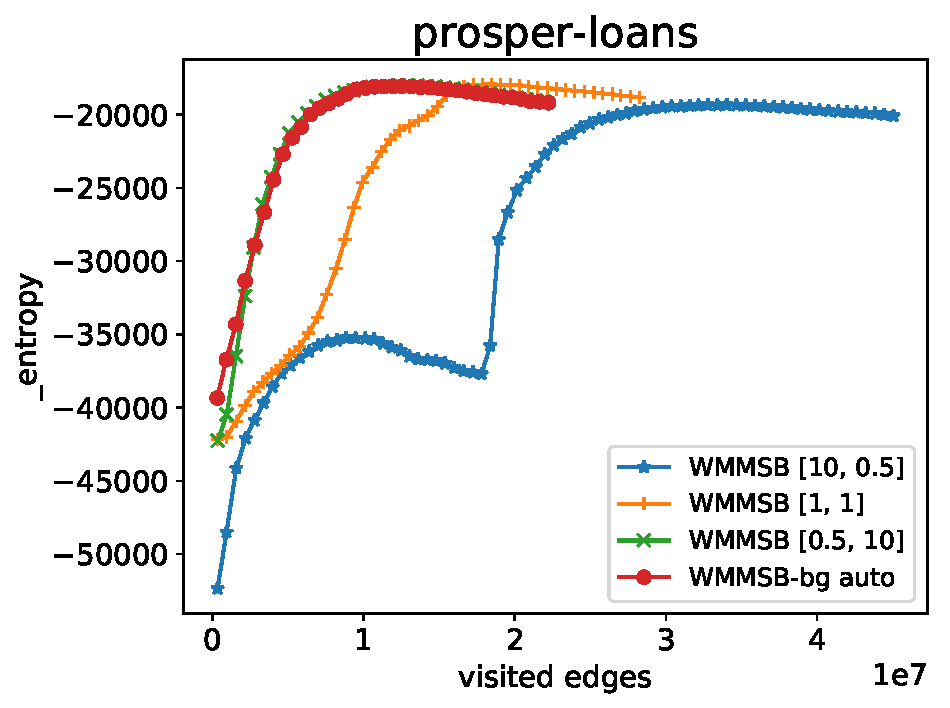
\includegraphics[width=0.32\textwidth]{fig/prosper-loans_fig__entropy}
\end{subfigure}                                                             
\begin{subfigure}                                                           
         \centering                                                         
      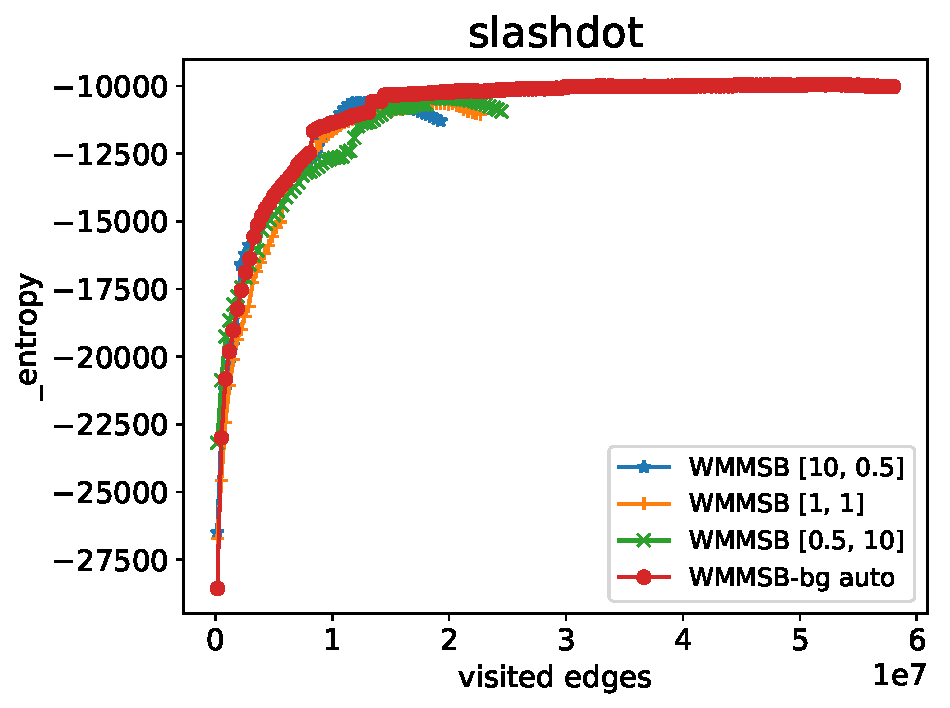
\includegraphics[width=0.32\textwidth]{fig/slashdot_fig__entropy}
\end{subfigure}                                                             
\caption{Log-likehood convergence for WMMSB and WMMSB-bg models. Three different set of hyper-parmeter are used for WMMSB.}


	\begin{subfigure}                                                                        
     \centering                                                                          
         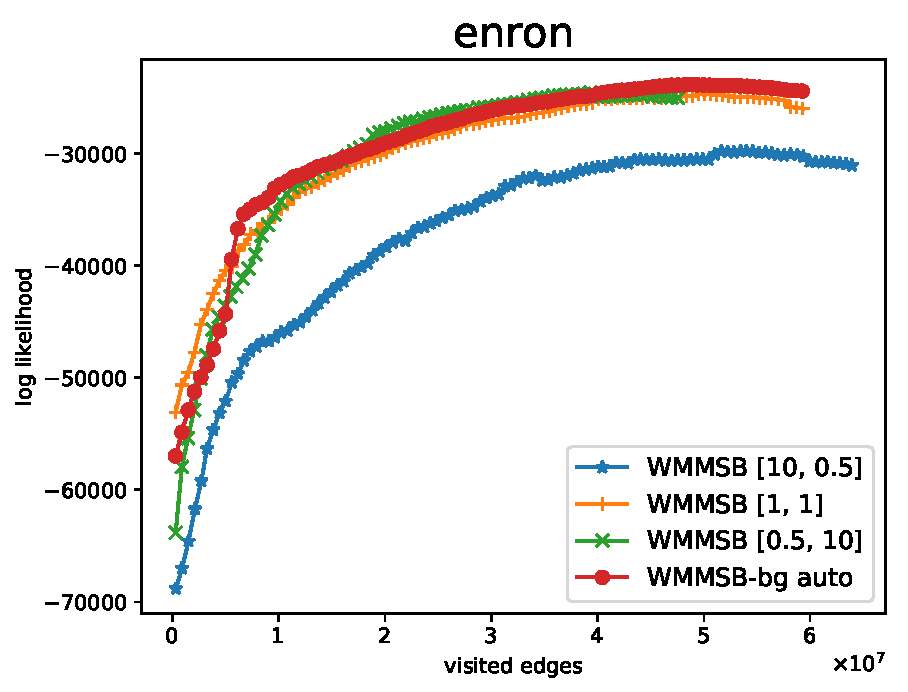
\includegraphics[width=0.32\textwidth]{fig/enron_fig__entropy__}
\end{subfigure}
\begin{subfigure}
         \centering
      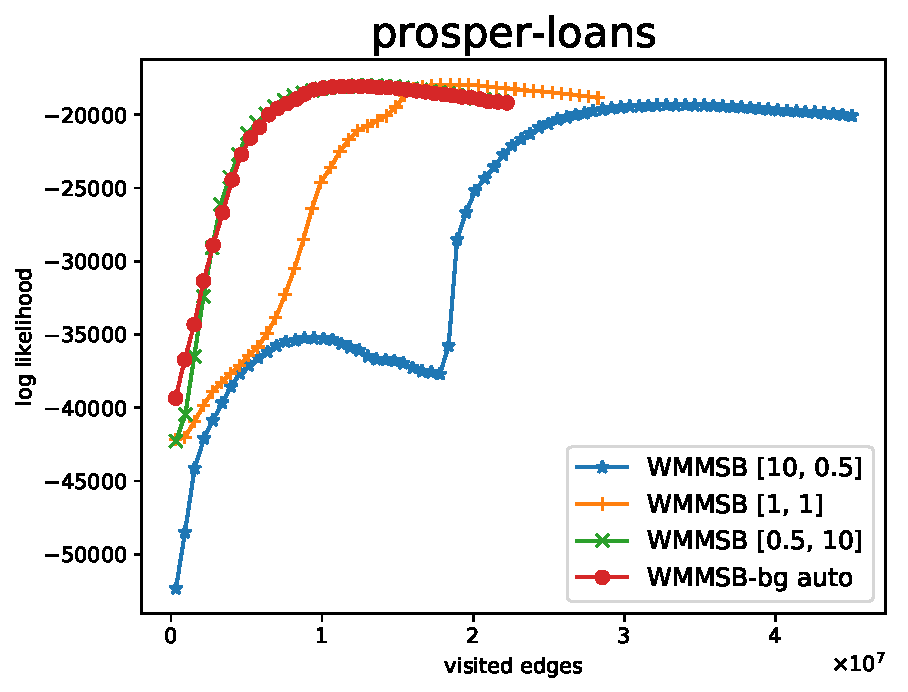
\includegraphics[width=0.32\textwidth]{fig/prosper-loans_fig__entropy__}
\end{subfigure}                                                             
\begin{subfigure}                                                           
         \centering                                                         
      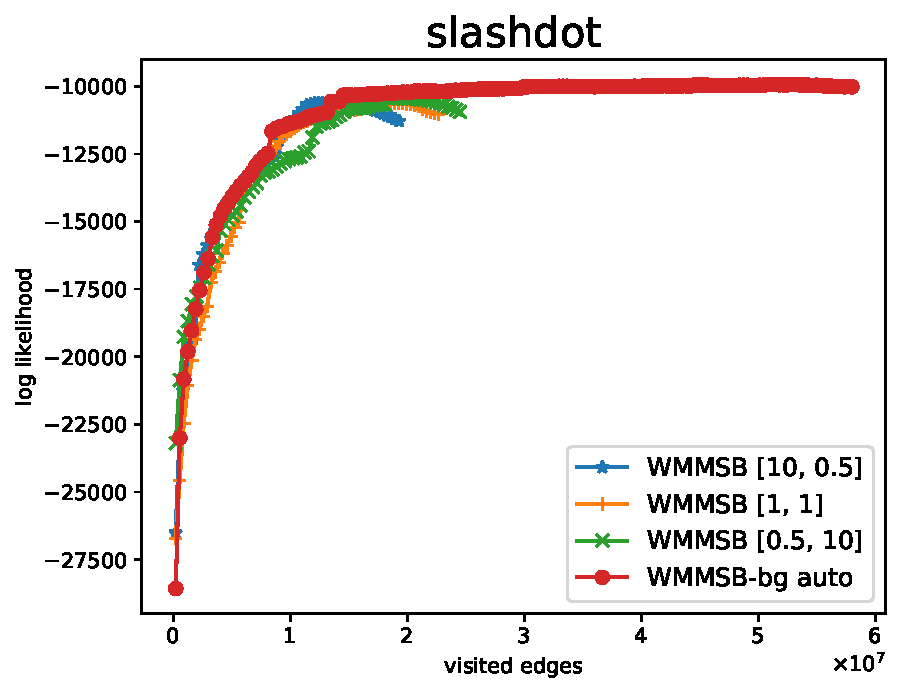
\includegraphics[width=0.32\textwidth]{fig/slashdot_fig__entropy__}
\end{subfigure}                                                             
\caption{Log-likehood convergence for WMMSB and WMMSB-bg models on a test set containing 20\% of the edges of the networks. Three different sets of hyperparmeters are used for WMMSB.}


    \label{fig:conv_entropy}
\end{figure*}

Table \ref{table:time} displays the inference time, in hours, of the different models on all datasets. The mixed-membership models, MMSB, WMMSB-bg,  SBM-ai, WSBM-ai-n and WSBM-ai-p are implemented in Python, while  EPM is implemented in Matlab and SBM and WSBM in C++ (with a Python wrapper \cite{peixoto_graph-tool_2014}). For all models, a hard limit was set at 25 hours for the inference time, to limit the computing cost. As one can observe, overall SBM (results in bold) is the fastest model and EPM (results in italics) the slowest one. Even though this latter model performs well in terms of weight prediction compared to stochastic block models, it can be more than 50 times slower than SBM. The mixed-membership model WMMSB-bg, which outperforms the other models in terms of weight prediction, can be up to 20 times faster than EPM. It is definitely slower than SBM but the difference remains reasonable as WMMSB-bg can be learned from millions of edges in less than 2 hours. Of course, the different implementations (python, Matlab, C++) render the comparison difficult and the results we are presenting should be understood with this difference in mind. They nevertheless reflect the behavior of the current, available implementations of the different models.

%%%%%%%%%%%%%%%%%%%%%%%%%%%%%%%%%%%%%%%%%%%%%%%%%%%%%%%%
%%%% Convergence of *MMSB SCVB inference
%%%%%%%%%%%%%%%%%%%%%%%%%%%%%%%%%%%%%%%%%%%%%%%%%%%%%%%%
\subsubsection{Convergence analysis} 

Lastly, Figure \ref{fig:conv_entropy} shows the evolution of the log-likelihood for the WMMSB and WMMSB-bg models on the test set for the enron, slashdot and proper-loans datasets. The number of visited edges corresponds to the number of edges used to infer the model (remember that the inference is stopped, for all models, when the likelihood  on the validation set no longer increases). We used three different sets of values for the hyperparameters $r$ and $p$ of WMMSB: $\{(10,0.1); (1,0.5); (0.5,0.66)\}$. Regardless of the values of these hyperparameters, one can observe that the augmented model WMMSB-bg converges to a better solution, in terms of likelihood, than the other models on enron and slashdot. The curve on slashdot further shows that the WMMSB models were stopped earlier than WMMSB-bg, illustrating the fact that this latter model, due to its additional prior assumptions, seems to be less prone to overfitting.









